\singlespacing

\chapter{Introduzione}

\section{Modulo \texttt{larcc}}
Nel modulo \texttt{larcc} vengono utilizzate delle rappresentazioni topologiche basilari, che includono alcuni comuni formati per le matrici sparse:
\begin{enumerate}
 \item CSR, \emph{Compressed Sparse Row}
 \item CSC, \emph{Compressed Sparse Column}
 \item COO, \emph{Coordinate Representation}
 \item BRC, \emph{Binary Row Compressed}
\end{enumerate}

\subsection{CSR (Compressed Sparse Row)}
Il formato \emph{Compressed Sparse Row} (CSR) memorizza una matrice $M$ di dimensione $m x n$ sparsa in forma di riga, utilizzando tre matrici 
unidimensionali $A$, $IA$, $JA$.\\
L'array $A$ contiene tutte i valori di $M$ diversi da zero, in ordine da sinistra a destra dall'alto verso il basso.\\
L'array $IA$ � di lunghezza $m + 1$, definito ricorsivamente nel modo seguente:
\begin{itemize}
 \item $IA_0 = 0$
 \item $IA_i = IA_{i - 1}$ + numero di elementi diversi da zero nella riga $i-1$ della matrice originale
\end{itemize}
Il terzo array, $JA$, contiene l'indice di colonna in $M$ di ciascun elemento di $A$. 

\subsection{CSC (Compressed Sparse Column)}
Il formato \emph{Compressed Sparse Column} (CSC) � simile a quello precedente, a eccezione del fatto che i valori vengono letti prima per colonna, 
viene memorizzato un indice di riga per ogni valore e vengono memorizzati i puntatori di colonna. 

\subsection{COO (Coordinate Representation)}
Il formato \emph{Coordinate Representation} (COO) memorizza una lista di tuple \emph{riga, colonna, valore}. Idealmente, le voci sono ordinate prima 
per indice di riga e poi per indice di colonna, per migliorare i tempi di accesso casuale.

\subsection{BRC (Binary Row Compressed)}
Il formato \emph{Binary Row Compressed} (BRC), nell'infrastruttura \texttt{larcc}, � il formato standard di matrice, utilizzato per rappresentare una 
matrice binaria solitamente sparsa.\\
Tale rappresentazione consiste in un array di array di interi, in cui gli array componenti non hanno necessariamente la stessa dimensione. Ogni array 
componente, corrispondente a una riga della matrice, contiene gli indici delle colonne in corrispondenza dei quali � memorizzato un $1$, mentre non 
viene tenuta traccia di eventuali zeri.

\section{Funzioni selezionate}
La scelta delle funzioni di cui realizzare la traduzione sequenziale da Python a Julia � stata effettuata in base alla frequenza con la quale le 
stesse venivano richiamate all'interno dei test del modulo. Di ognuna di queste funzioni selezionate, vengono riportati una breve descrizione del 
comportamento, il codice originario in Python, la relativa traduzione in Julia, la versione parallela e i tempi di esecuzione.

\vspace{1 cm}

\begin{tabular}{p{4.8 cm} p{4.8 cm} p{4.8 cm}}
\toprule
\textbf{API}			& \textbf{Locali} 		& \textbf{Funzioni esterne} 	\\
\midrule
\texttt{csrCreate}		&				& 				\\
\texttt{brc2Coo}		&				& 				\\
\texttt{coo2Csr}		&				& 				\\
\texttt{triples2mat}		&				& 				\\
\texttt{csr2DenseMatrix}	&				& 				\\
\texttt{csrGetNumberOfRows}	&				& 				\\
\texttt{csrGetNumberOfColumns}	&				& 				\\
\texttt{larModelNumbering}	& \texttt{larModelNumbering0} 	& \texttt{cellNumbering}	\\
\texttt{larFacets}		&				& 				\\
\texttt{setup}			&				& 				\\
\texttt{larCellAdjacencies}	&				& 				\\
\texttt{matrixProduct}		&				& 				\\
\texttt{csrTranspose}		&				& 				\\
\texttt{csrPredFilter}		&				& 				\\
\texttt{mkSignedEdges}		& 				& 				\\
\bottomrule
\end{tabular}

\vspace{1 cm}

\section{Grafico delle dipendenze tra funzioni}

\begin{figure}[H]
  \centering 
  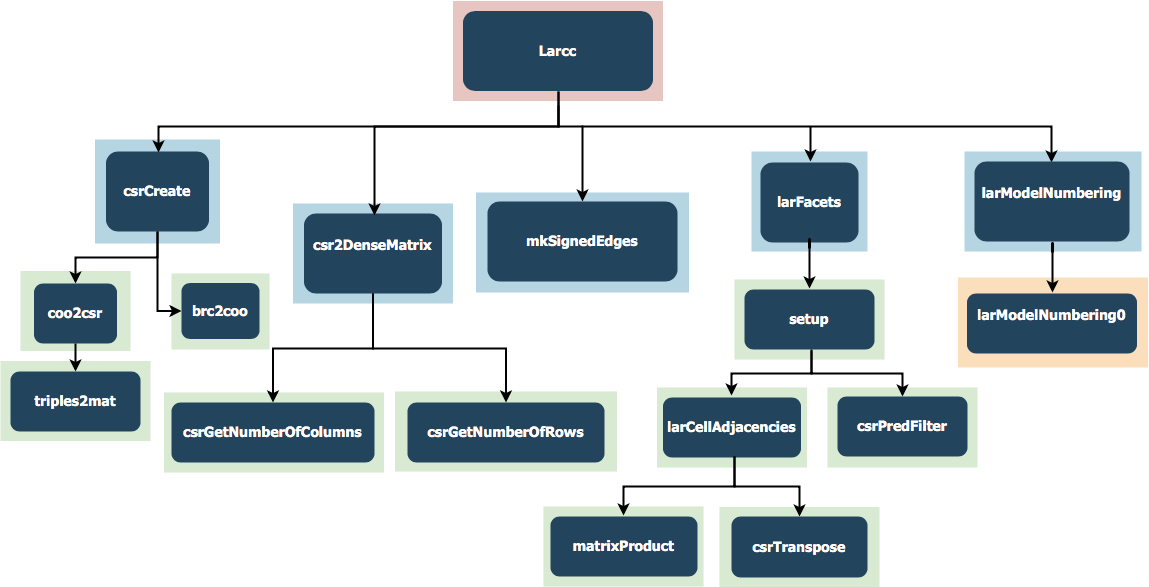
\includegraphics[width=1\columnwidth]{immagini/Larcc}
\end{figure}

\vspace{1 cm}

\section{Tempi di esecuzione}
Per calcolare i tempi di esecuzione delle funzioni, sia in versione seriale sia parallelizzata, sono state utilizzate la macro \texttt{@elapsed} e la 
macro \texttt{@timev} (versione \emph{verbose} della macro \texttt{@time}). La prima resituisce soltanto il tempo in secondi, la seconda restituisce 
anche la quantit� di memoria allocata. \\

\noindent Dal momento che alla prima chiamata di \texttt{@elapsed f(args)} o \texttt{@timev f(args)} la funzione \texttt{f} deve essere compilata 
prima che eseguita, il primo utilizzo delle macro non deve essere considerato, perch� il tempo di esecuzione sar� sicuramente peggiore del normale.
